\chapter[\texorpdfstring{The $^\text{12}$B\lowercase{($d$,$p$)} Measurement}{The 12B(d,p) Measurement}]{\texorpdfstring{The $^\mathbf{12}$B($d$,$p$) Measurement}{The 12B(d,p) Measurement}}
\label{rib_com}
\section{Introduction}
The commissioning experiment described in the previous chapter served to demonstrate the validity of the HELIOS concept.  The first groundbreaking physics measurement made with the HELIOS spectrometer was the study of the $d$($^{12}$B,$p$)$^{13}$B reaction conducted in March, 2009.  The details of this experiment are reported in Ref.~\cite{Schiffer_2010}; this chapter summarizes those results. This experiment was a repeat measurement of the reaction discussed in Chapt.~\ref{standards}.  The measurement needed to be repeated because the previous experiment, which was carried out using conventional detector geometry, was unable to resolve a pair of states in $^{13}$B separated by $\Delta E_x=199$\,keV.  Separation of this doublet would provide a strict test of the resolution performance of the spectrometer.  This experiment was the first reaction study using HELIOS with a radioactive beam and is considered the first ``experiment'' with HELIOS.  

\section{Experimental Setup}
The method of beam production used in this experiment is identical  to those described in Chapt.~\ref{standards}~\cite{Lee_2010}.  Briefly, a 81\,MeV primary beam of $^{11}$B bombarded a cryogenic gas cell filled with deuterium gas to produce in-flight a 75\,MeV $^{12}$B secondary beam.  The primary beam had an intensity of 50\,pnA ($3.1\times 10^{11}$ ions/s) and the secondary beam had an intensity of $6\times 10^5$\,ions/s on target.  A 73\,$\mu$g/cm$^2$ thick CD$_2$ target was used, placed at the center of the magnet at $z=0$\,mm.  For the duration of the measurement the solenoid was set to a central field value of $\mathscr{B}_0=1.04$\,T and the array was placed upstream of the target at a target-to-detector separation of $\Delta z = 368.7$\,mm.  Table~\ref{b_coverage} shows the corresponding detector coverage for both reactions.  For recoil detection, a 4-quadrant $\Delta E$-$E$ telescope array was placed 1,032\,mm downstream from the target (as shown in Fig.~\ref{schematic}), covering $\theta_\mathrm{lab}=0.5^\circ$--2.9$^\circ$.  The $\Delta E$ energy loss detectors were nominally 80\,$\mu$m thick (the actual thicknesses ranged from 79--81\,$\mu$m) and the $E$ residual energy detectors were nominally 500\,$\mu$m thick (493--496\,$\mu$m).  The method of recoil detection is described in Chapt.~\ref{recoil}.  By gating the proton spectra on both the 63.0\,ns time-of-flight and the detection of recoiling heavy ion, the measured backgrounds are largely suppressed. 

\begin{table}%
\centering
\begin{tabular}{cd{2}rrcrrcc}
Set&\multicolumn{1}{c}{$\Delta z$}
&\multicolumn{2}{c}{$\theta_\mathrm{lab}$}&&\multicolumn{2}{c}{$\theta_\mathrm{cm}$}&$\Delta \cos(\theta_\mathrm{cm})$&$\Delta \Omega$\\ \cline{3-4} \cline{6-7}
&\multicolumn{1}{c}{(mm)}&\multicolumn{1}{c}{$\theta_1$}&\multicolumn{1}{c}{$\theta_2$}&&\multicolumn{1}{c}{$\theta_1$}&\multicolumn{1}{c}{$\theta_2$}&&(sr)\\
\hline \hline
$^{11}$B & 368.7&  111.7&151.6&&31.3&10.4&0.113&0.34\\
$^{12}$B & 368.7&  114.3&154.4&&28.9&5.4&0.120&0.36\\
 \hline
\end{tabular}
\caption[Detector positions and solid angle coverage for the $^{11,12}$B($d$,$p$) measurement]{Detector positions and solid angle coverage for the $^{11,12}$B($d$,$p$) measurement.  Since the ground-state transition was outside of the acceptance for both data sets, the coverage of a state which spans the array is given; the 2.62\,MeV state in $^{12}$B and the 3.48\,MeV state in $^{13}$B.  The target and array remained at the same position for both measurements.}
\label{b_coverage}
\end{table}

\section{Results}
\subsection{Energy Resolution}
Fig.~\ref{b11_spec} shows the characteristic energy versus position spectrum for the $^{11}$B($d$,$p$)$^{12}$B stable beam calibration measurement.  The spectrum is gated on two event criteria.  First the flight times consistent with single-orbit protons (63\,ns).  As was shown with the data from the $^{28}$Si($d$,$p$) reaction in Fig.~\ref{cezg_350}, gating on time alone is insufficient to eliminate the background due to fusion-evaporation reactions  of involving the $^{12}$C in the CD$_2$ target.  The second gating criterion in Fig.~\ref{b11_spec} is the requirement of a coincidence measurement of the recoiling $^{12}$B ion in the heavy recoil detector.  This added step dramatically reduces the background (\textit{cf}. Fig.~\ref{cezg_350}).  
\begin{figure}[t]
\centering
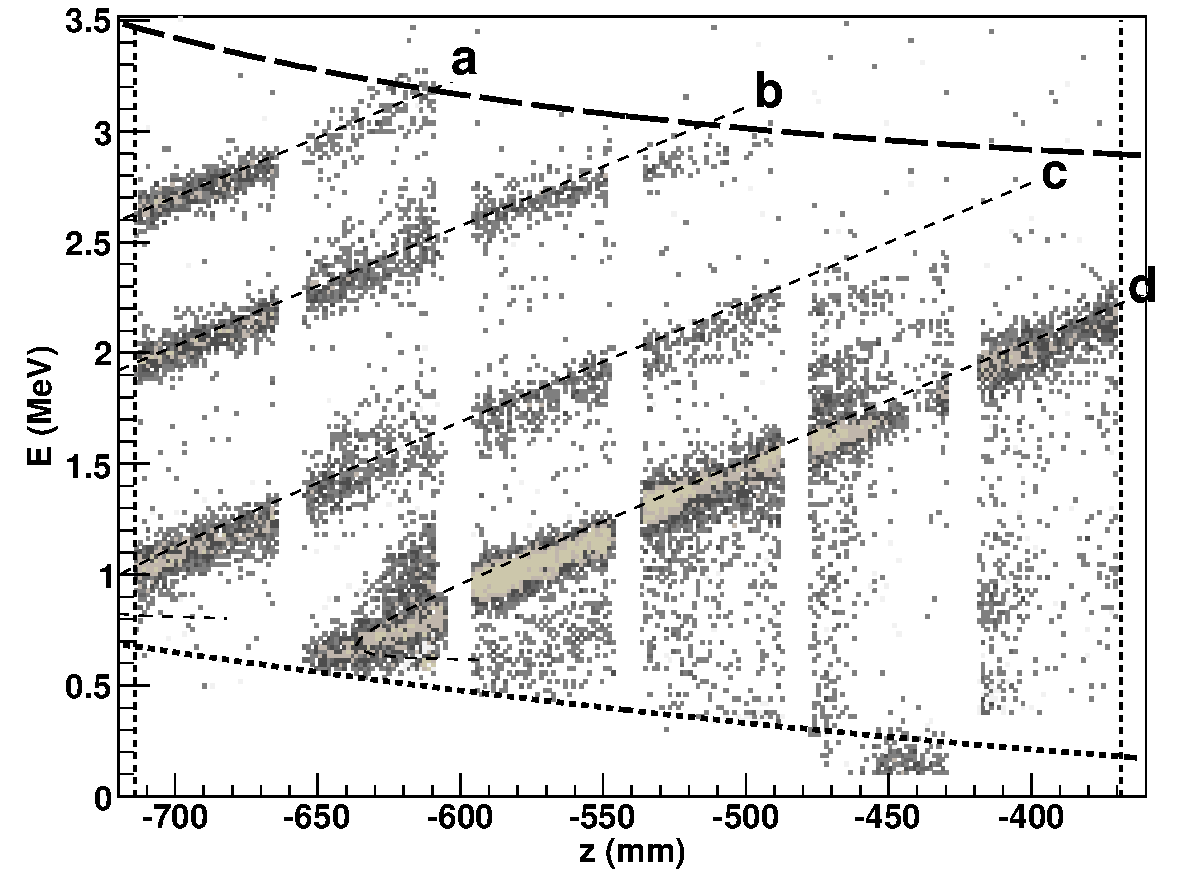
\includegraphics[width=\columnwidth,keepaspectratio]{cB11_bw.eps}%
\caption[Energy vs. position spectrum for protons from the $^{11}$B($d$,$p$) reaction]{Energy vs. position spectrum for protons from the $^{11}$B($d$,$p$) reaction.  Events are gated on a time-of-flight consistent with single-orbit protons and on coincidence with the recoiling $^{12}$B identified in the heavy ion recoil detector.  The thin dashed lines indicate the analytically calculated positions of the kinematic groups;  the excitation states are labeled (a) 0.95\,MeV ($J^\pi=2^+$), (b) 1.62\,MeV ($J^\pi=2^-$), (c) 2.62\,MeV ($J^\pi=1^-$) (d) 3.39\,MeV ($J^\pi=3^-$). The bold wide-dashed line corresponds to the acceptance limit imposed by the solenoid bore.  This data appear in a similar form in Ref.~\cite[Fig.~2]{Schiffer_2010}. }%
\label{b11_spec}%
\end{figure}

The ground state of $^{11}$B has a spin and parity of $J^\pi=3/2^-$.  The $\ell_n=0$ transition populates states corresponding to $J=3/2\pm1/2$, which are the second- and third-excited states.  Both of these states were populated in this reaction; the $J^\pi=2^-$ state has an excitation energy of $E_x=1.67$\,MeV (b in Fig.~\ref{b11_spec}) and the $J^\pi=1^-$ state has an excitation energy of $E_x=2.62$\,MeV (c).  Fig.~\ref{b11b12_spec_helios} shows the excitation energy spectrum from this measurement. The $Q$-value resolution was about 100\,keV.   The $\Delta E_x=102$\,keV doublet near 2.7\,MeV  is unresolved.  The angular distributions of the 2.62 and 3.39\,MeV states are shown in Fig.~\ref{b12angdist}.  

Fig.~\ref{b12_spec} shows a simulated energy versus position spectrum for the $^{12}$B($d$,$p$) reaction, requiring coincidence with the recoiling $^{13}$B nucleus.  As the simulation shows, using similar resolution parameters as those discussed in Chapt.~\ref{simulation}, the $\Delta E_x=199$\,keV double near 3.6\,MeV should be able to be resolved in this measurement; and indeed it was.  Fig.~\ref{b11b12_spec_helios} shows the excitation energy spectrum from this measurement.  Comparing this figure to Fig.~\ref{b11b12_spec} is a direct, practical demonstration of the enhanced $Q$-value resolution provided by the HELIOS technique.  This measurement made with HELIOS had $3\times$ better resolution than the previous measurement made using conventional detector geometry.

\begin{figure}[t]
\centering
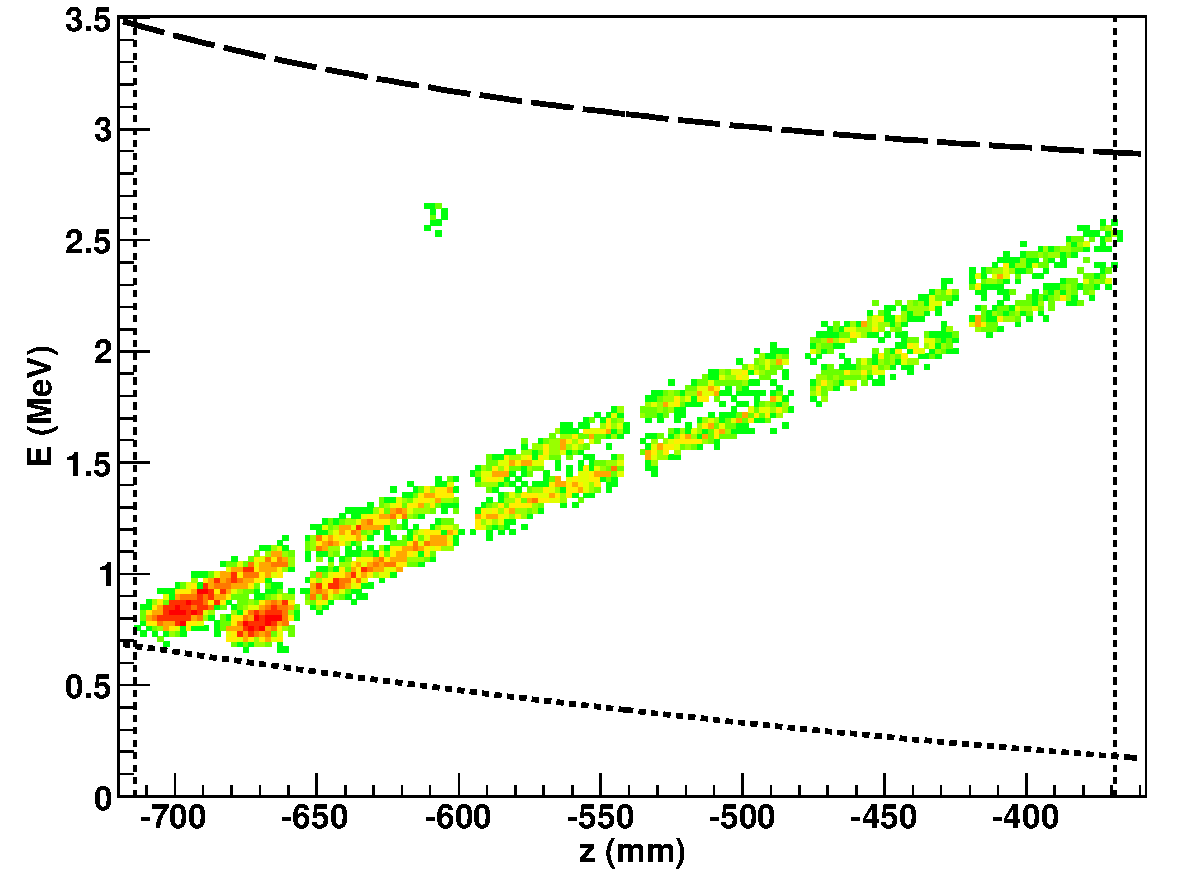
\includegraphics[width=\columnwidth,keepaspectratio]{cB12.eps}%
\caption[Simulated proton spectrum of the $^{12}$B($d$,$p$) reaction. ]{Simulated proton spectrum of the $^{12}$B($d$,$p$) reaction.  The 3.48\,MeV (upper) and 3.69\,MeV (lower) kinematic groups are plotted with a simulated coincidence requirement with the recoiling $^{13}$B nucleus.  Dashed lines indicate the acceptance region of the spectrometer.}%
\label{b12_spec}%
\end{figure}

\subsection{Angular Distributions}\label{b12_ang}
The two states with the most statistics from the $^{11}$B($d$,$p$)$^{12}$B reaction---the 2.62\,MeV and 3.39\,MeV excited states---were used to calibrate the efficiency of the detector array.  The 3.39\,MeV excited state was populated with over 4$\times$ the statistics of any other state; this state was used to calibrate most of the array.  However, examination of Fig.~\ref{b11_spec} reveals that the 3.39\,MeV state (labeled b in the figure) does not extend onto detector position 1.  This position was calibrated with the 2.62\,MeV excited state (c in the figure).    The array is binned into equal ranges of $\Delta z$ with each bin corresponding to one detector.  The equal ranges of $\Delta z$ are equivalent to equal ranges of $\Delta \cos(\theta_\mathrm{cm})$, in this case $\Delta \cos(\theta_\mathrm{cm})=0.019$ or 14.5\,msr.%\pagebreak

The angular distributions from the $^{11}$B($d$,$p$) reaction were fitted to the results of DWBA calculations carried out using three different parameter sets that had previously been used to reproduced the angular distributions for this reaction~\cite{Perey_1963, Schiffer_1967, Corrigan_1972}.  For each solid angle bin (one per detector position), an efficiency factor equal to the ratio of DWBA/data was produced.  These fixed efficiency factors were then applied uniformly to all of the data.  The results of this procedure are shown in Fig.~\ref{b12angdist}.  However, even without applying this technique, the 3.48\,MeV state displays the characteristic behavior of an $\ell_n=0$.  Fig.~\ref{doublet} shows the excitation energy spectrum of the 3.6\,MeV doublet for two different angle ranges.  In the top panel of the figure, counts from the entire array are used.  In the bottom panel of the figure, counts in the range of $\theta_\mathrm{cm}=5^\circ$--$17^\circ$ have been excluded (half the array).  The dramatic reduction of counts in the 3.48\,MeV peak when excluding forward angles is an illustration of the forward-peaked nature of the 3.48\,MeV state, which is consistent with a $\ell_n=0$ transfer.

\begin{figure}%
\centering
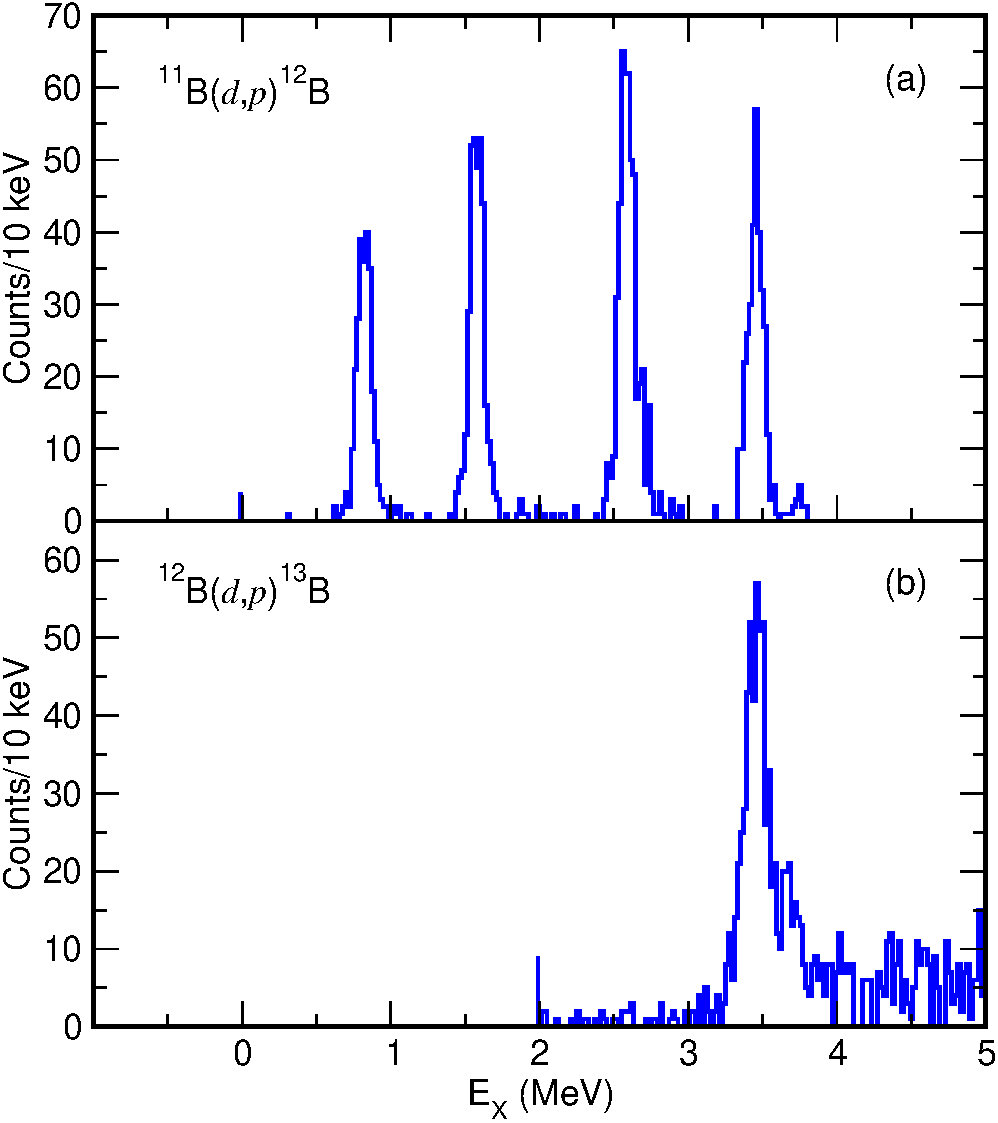
\includegraphics[height=0.45\textheight,width=\columnwidth,keepaspectratio]{ex_comparison}%
\caption[Excitation energy spectra from the $^{11,12}$B($d$,$p$) reactions]{Excitation energy spectra from the (top) $^{11}$B($d$,$p$) and (bottom) $^{12}$B($d$,$p$) reactions, as reported in Ref.~\cite{Schiffer_2010}. Comparing this figure to Fig.~\ref{b11b12_spec} (on page~\pageref{b11b12_spec}) is a direct, practical demonstration of the enhanced $Q$-value resolution provided by the HELIOS technique.  Figure from Ref.~\cite{Wuosmaa_2011PC}.}%
\label{b11b12_spec_helios}%
\end{figure}

\pagebreak

\begin{figure}
\centering
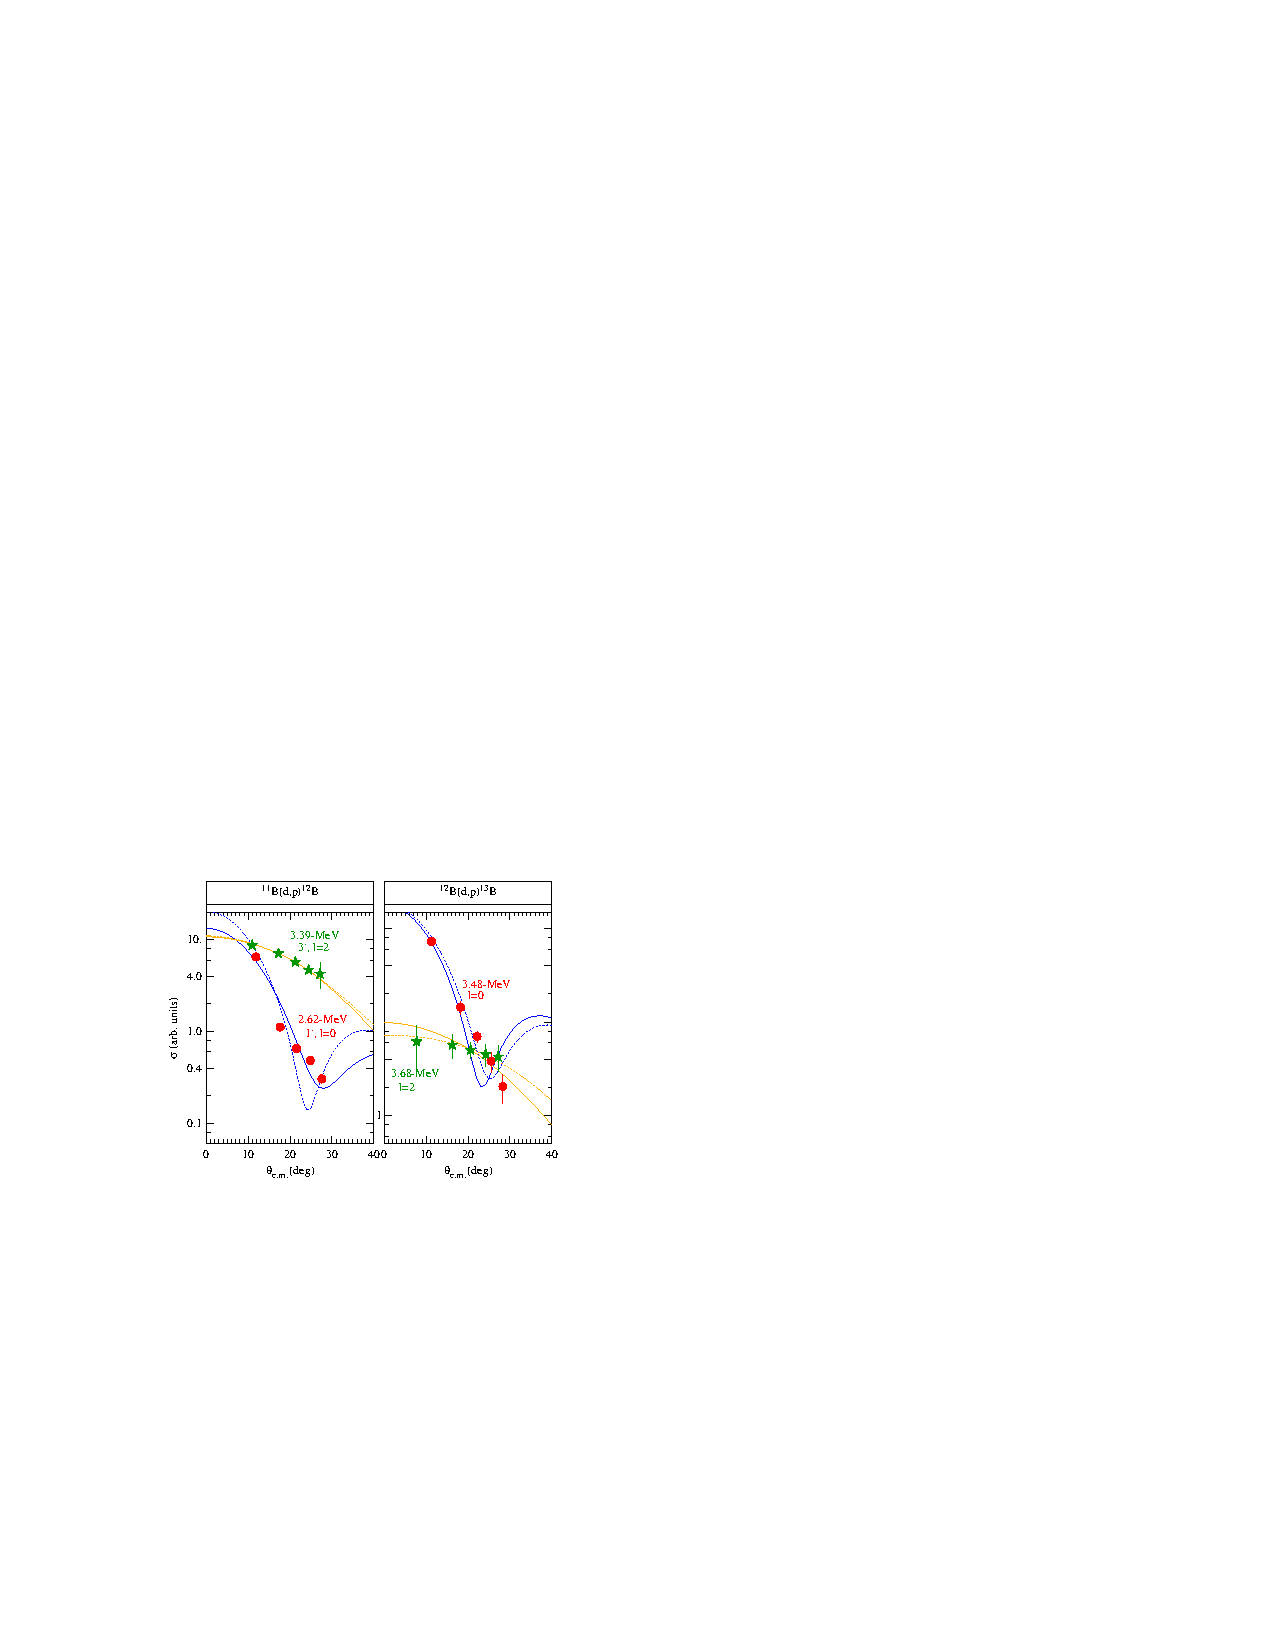
\includegraphics[height=0.38\textheight,width=\columnwidth,keepaspectratio]{Schiffer_2010-fig3}%
\caption[Angular distributions from the $^{11,12}$B($d$,$p$) reactions]{Angular distributions from the (left) $^{11}$B($d$,$p$) and (right) $^{12}$B($d$,$p$) reactions as reported in Ref.~\cite{Schiffer_2010}.  The characteristic shape of the $\ell_n=2$ angular distribution of the 3.39\,MeV in $^{12}$B was used to calibrate the efficiency of the detector array.  Applying this calibration to the $^{13}$B data reveals the clear $\ell_n=0$ character of the 3.48\,MeV state and the $\ell_n=2$ character of the 3.68\,MeV state.  Figure taken from Ref.~\cite[Fig.~3]{Schiffer_2010}.}%
\label{b12angdist}%
\end{figure}

\begin{figure}[t]
\centering
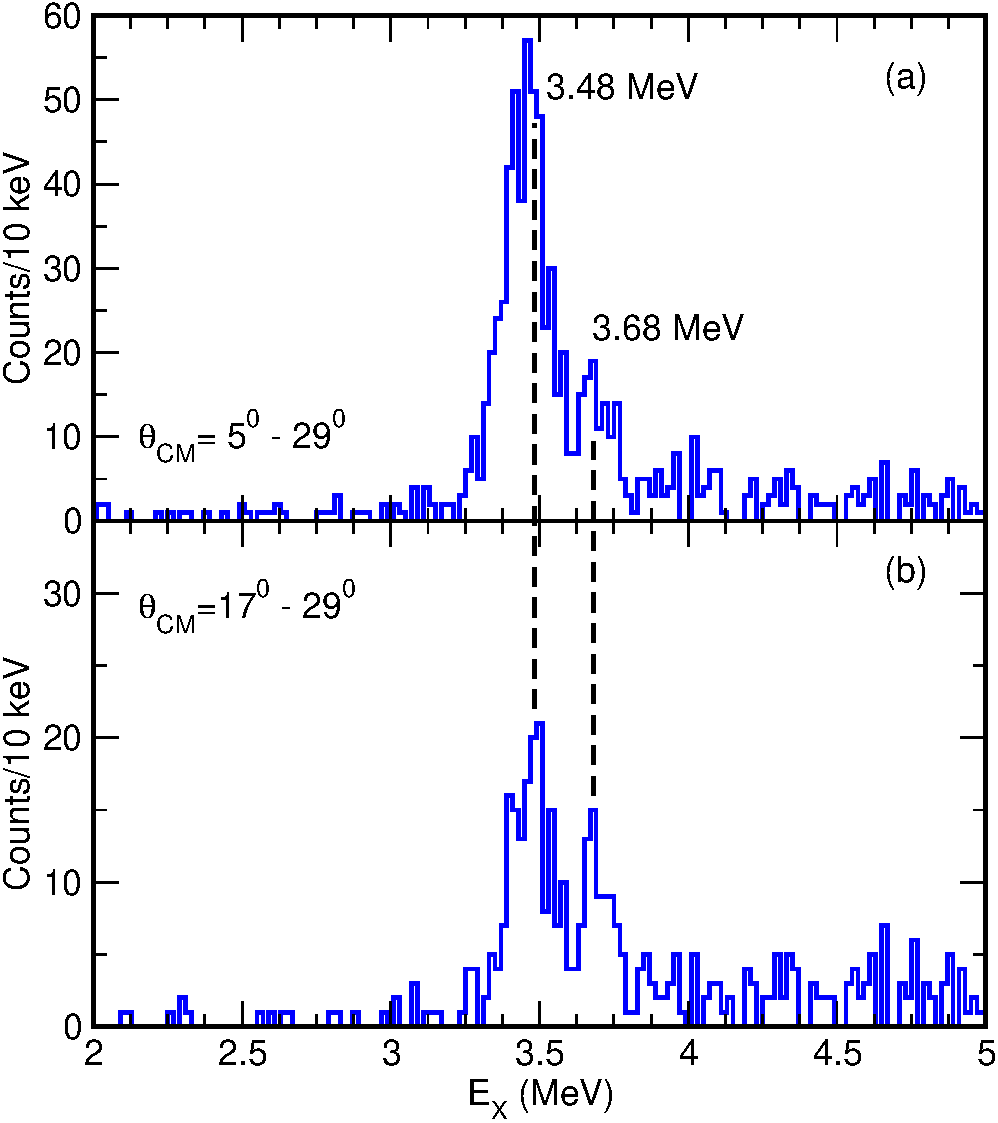
\includegraphics[height=0.45\textheight,width=0.5\columnwidth,keepaspectratio]{doublet}%
\caption[Excitation energy spectrum of the 3.6\,MeV doublet for different angular ranges]{Excitation energy spectrum of the 3.6\,MeV doublet for two different angular ranges.  Panel (a) includes counts from the entire array (detector positions 1--6), corresponding to a center-of-mass range of $\theta_\mathrm{cm}=5^\circ$--$29^\circ$. Panel (b) is includes counts from only detectors 3--6, corresponding to a center-of-mass range of $\theta_\mathrm{cm}=17^\circ$--$29^\circ$.  The dramatic reduction of counts in the 3.48\,MeV peak when excluding forward angles is an illustration of the forward-peaked nature of the 3.48\,MeV state, which is consistent with a $\ell_n=0$ transfer.  Figure from Ref.~\cite{Wuosmaa_2011PC}.}%
\label{doublet}%
\end{figure}

%\chapter[\texorpdfstring{Angular Distributions of the $^\text{12}$B\lowercase{($d$,$p$)} Measurement}{Angular Distributions of the 12B(d,p) Measurement}]{\texorpdfstring{Angular Distributions of the \newline $^\mathbf{12}$B($d$,$p$) Measurement}{Angular Distributions of the 12B(d,p) Measurement}}
\label{badang}
Following the discussion of \ref{b12_ang}, this chapter further details the method of analysis used for determining the angular distributions of $^{11}$B($d$,$p$) and $^{12}$B($d$,$p$).

The two states with the most statistics---the 2.62\,MeV and 3.39\,MeV excited states---were used to to calibrate the efficiency of the detector array.  The 3.39\,MeV excited state was populated with over 4$\times$ the statistics of any other state; this state was used to calibrate most of the array.  However, examination of Fig.~\ref{b11_spec} reveals that the 3.39\,MeV state (labeled d in the figure) does not extend onto detector position 1.  This position was calibrated with the 2.62\,MeV excited state (c in the figure).  Fig.~\ref{b12angdist2} illustrates the method of efficiency calibration. Following the procedure described in the previous chapter, the array is binned into equal ranges of $\Delta z$; in this case, each bin corresponds to half a detector detector.  The equal ranges of $\Delta z$ are equivalent to equal ranges of $\Delta \cos(\theta_\mathrm{cm})$, in this case $\Delta \cos(\theta_\mathrm{cm})=0.009$ or 2.3\,msr.  In the top panel of the figure, the un-normalized angular distribution is plotted with a DWBA calculation fitted to the points. 

In the lower panel in the figure, the data have been scaled by a ratio of DWBA/data.  Notice that all of the points in the 3.39\,MeV angular distribution, corresponding to detectors 2--6, lie on the DWBA calculation.  In addition, the first two points of the 2.62\,MeV angular distribution, corresponding to detector 1, also line up with the DWBA calculation. 

\begin{figure}%
\centering
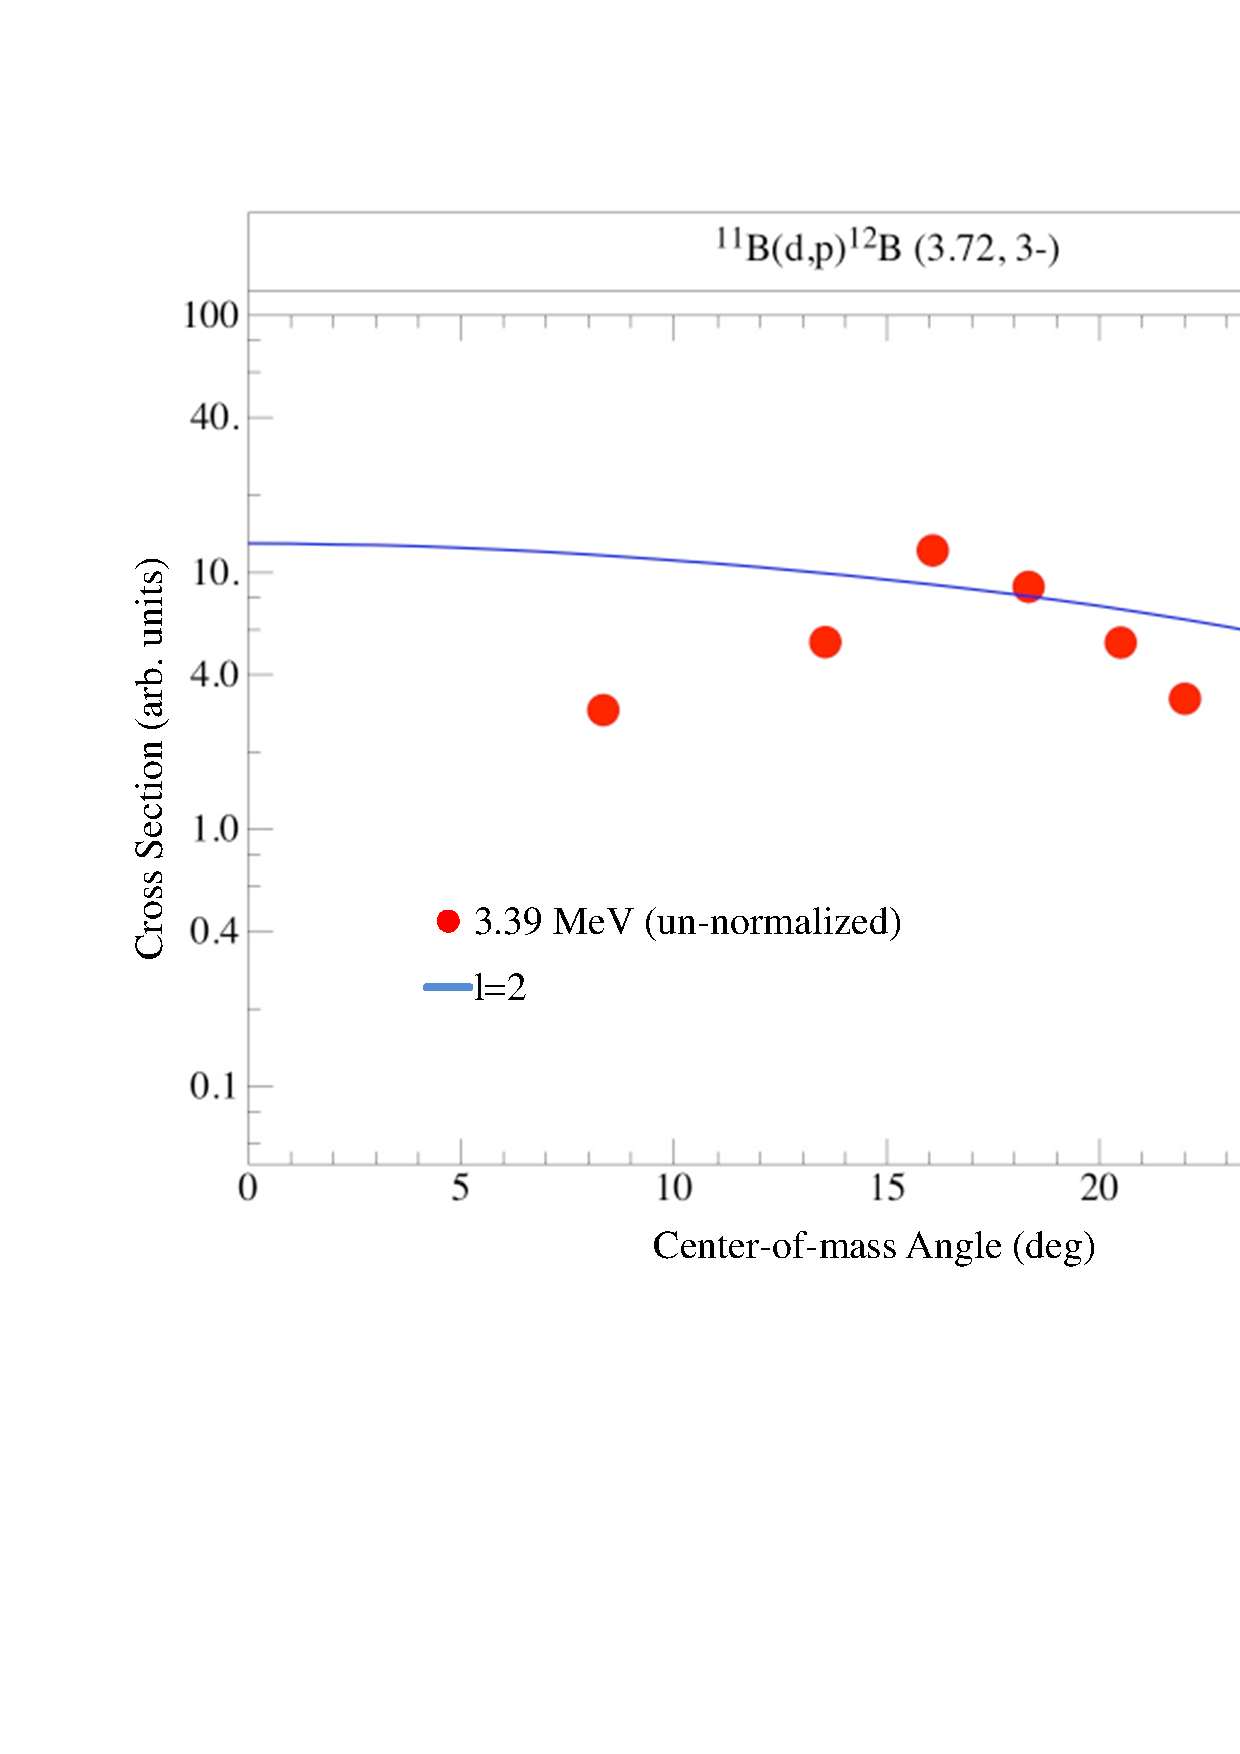
\includegraphics[height=0.45\textheight,width=\columnwidth,keepaspectratio]{More_Figures/b12_unnorm}\\
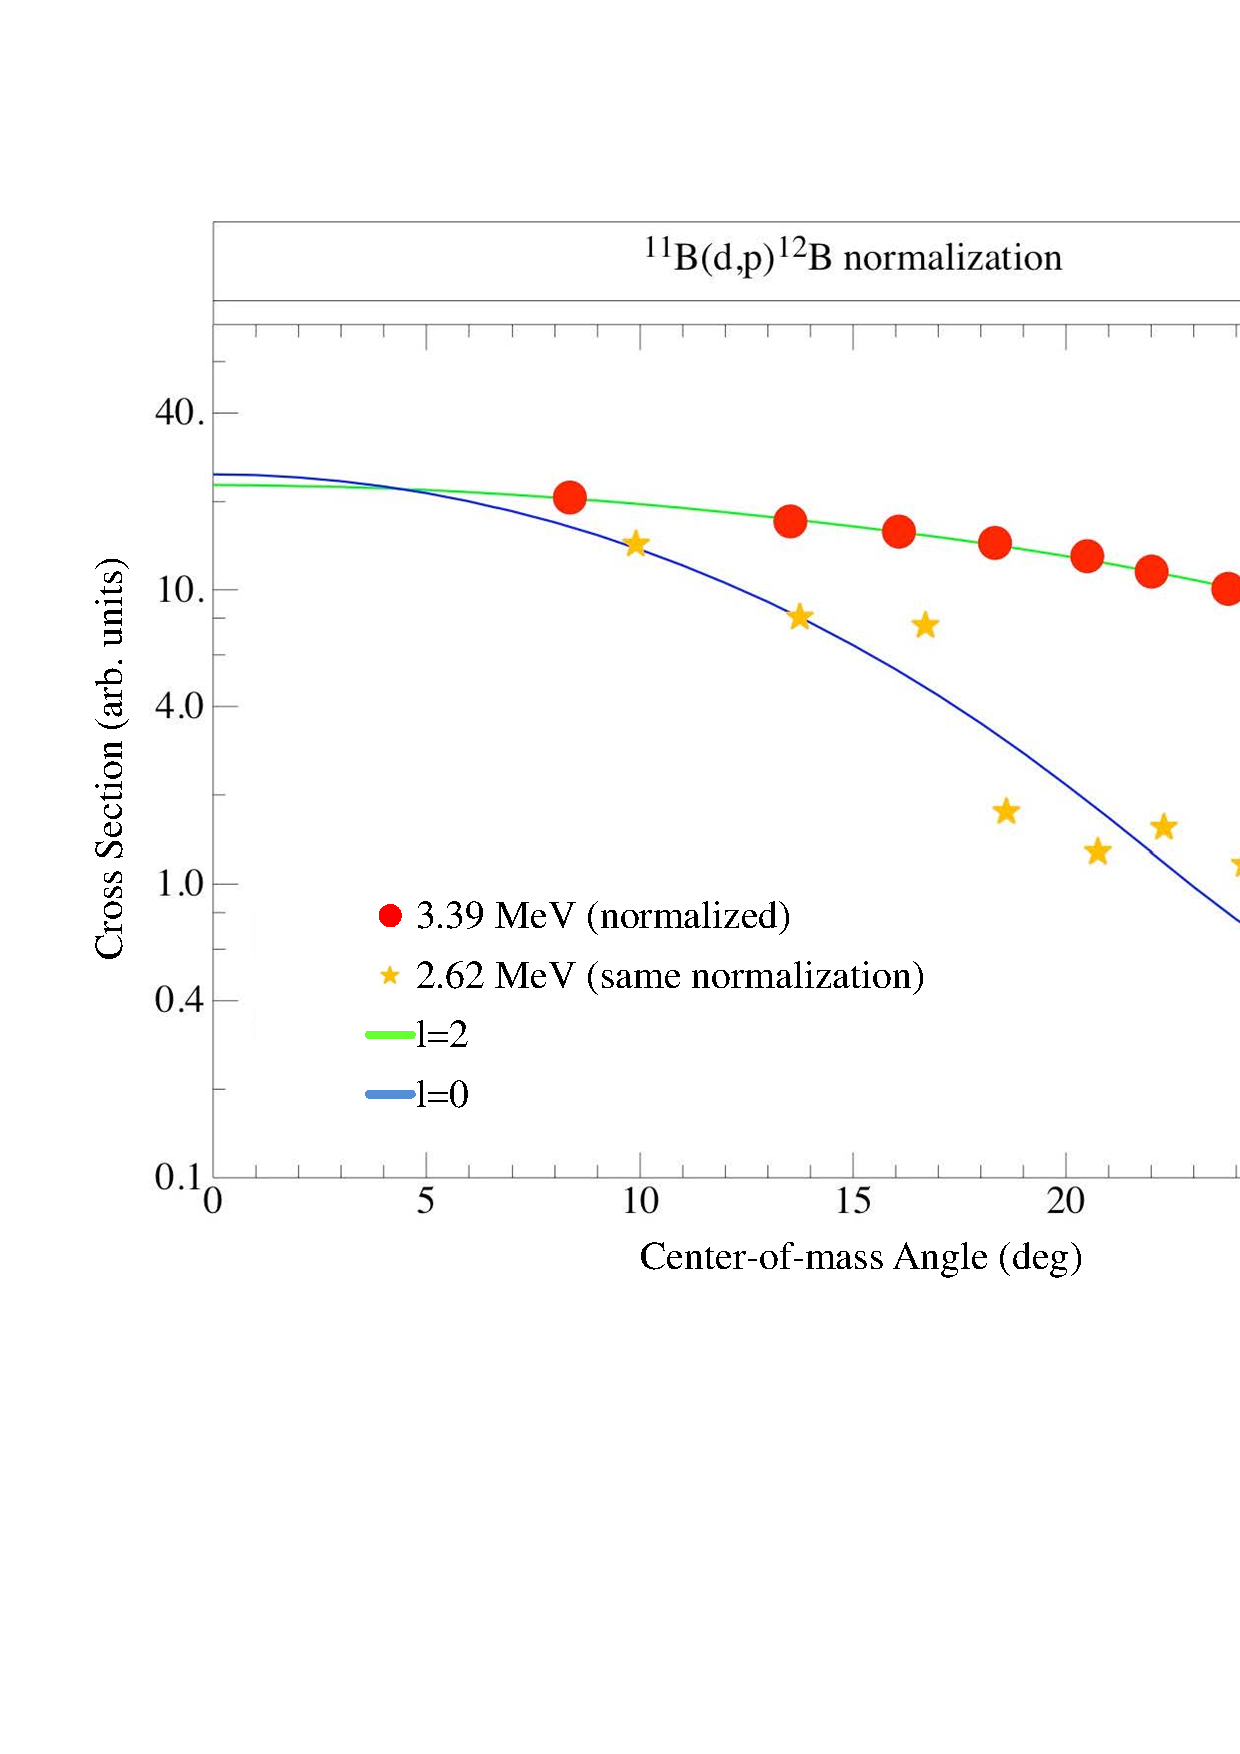
\includegraphics[height=0.45\textheight,width=0.98\columnwidth,keepaspectratio]{More_Figures/b12_norm}%
\caption[Illustration of the efficiency calibration technique]{Illustration of the efficiency calibration technique.  In the top panel the angular distribution of the 3.39\,MeV state ($\ell_n=2$) is fitted with a DWBA calculation.  In the bottom figure, the data points have been scaled by (DWBA/data), with each bin having the same efficiency correction. Figure annotated from Ref.~\cite{Schiffer_2009PC}.}%
\label{b12angdist2}%
\end{figure}

\begin{figure}[p]
\centering
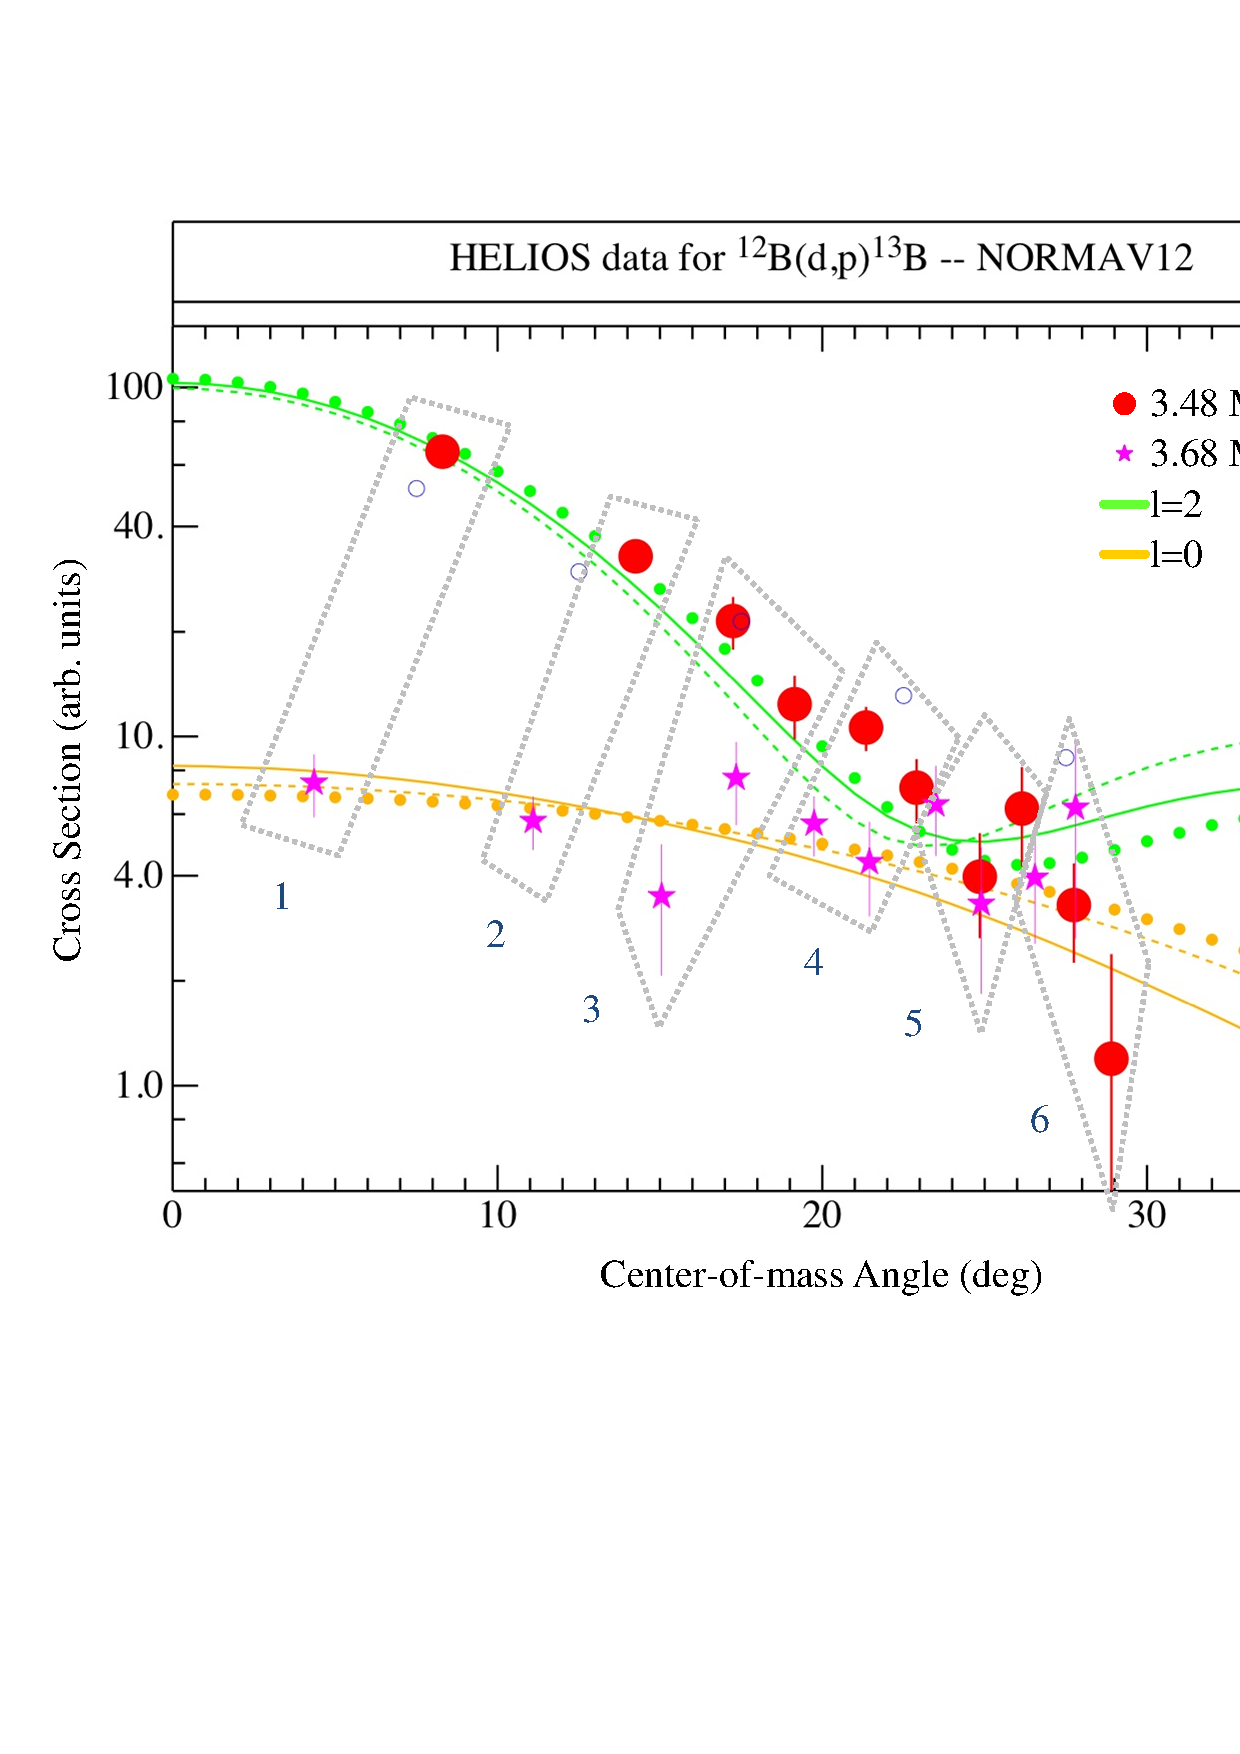
\includegraphics[height=0.4\textheight,width=\columnwidth,keepaspectratio]{More_Figures/b13}%
\caption[Angular distribution of of the $^{12}$B($d$,$p$) reaction]{Angular distribution of of the $^{12}$B($d$,$p$) reaction using the normalization derived from the $^{11}$B($d$,$p$) reaction.  DWBA calculations have been fit to the data using three different optical model parameters sets, discussed in Ref.~\cite{Schiffer_2010}. The quadrilateral boxes group data points corresponding to individual detector positions.  Please note that this is an annotated figure from a private communication~\cite{Schiffer_2009PC} and should be considered for illustrative purposes only.  The value of the angles plotted correspond to a target-to-detector separation of $\Delta z = 428$\,mm, which is consistent with using detector positions 1--5 only; however, as indicated in the figure, all six detector position are represented. This minor computational error is corrected in Ref.~\cite{Schiffer_2010}.
}%
\label{b13angdist}%
\end{figure}

